\definecolor{zzttqq}{rgb}{0.15,0.35,0.15}

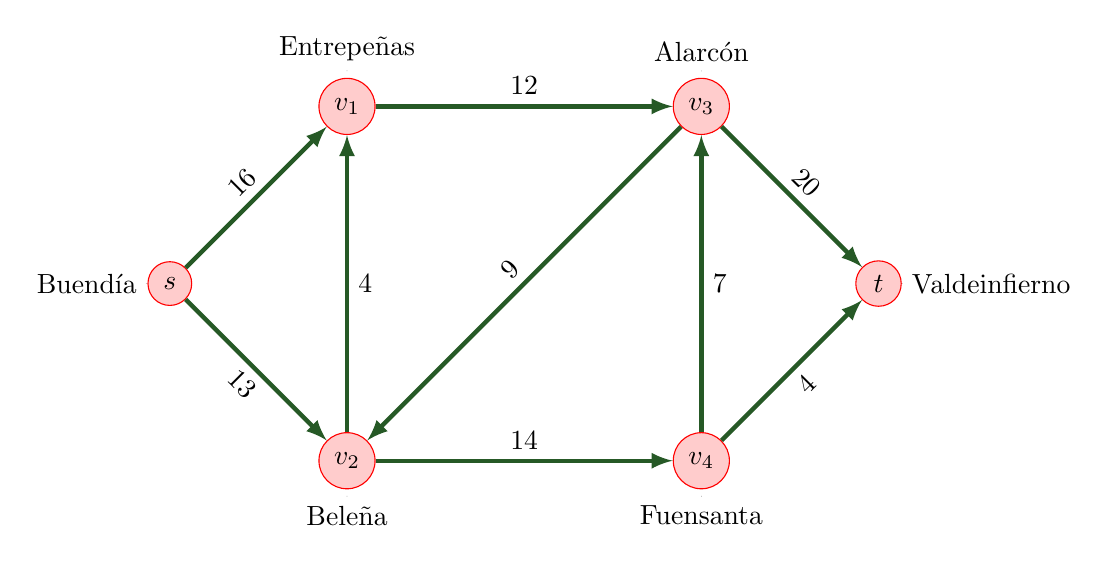
\begin{tikzpicture}[x=1.5cm, y=1.5cm]
	\fill (-3.2,0) circle (0.1pt)node[anchor=east] {Buendía};
	\fill (3.2,0) circle (0.1pt)node[anchor=west] {Valdeinfierno};
	\fill (-1.5,1.8) circle (0.1pt)node[anchor=south] {Entrepeñas};
	\fill (-1.5,-1.8) circle (0.1pt)node[anchor=north] {Beleña};
	\fill (1.5,1.8) circle (0.1pt)node[anchor=south] {Alarcón};
	\fill (1.5,-1.8) circle (0.1pt)node[anchor=north] {Fuensanta};
    \node[circle,draw=red,fill=red!20!] (v1) at (-1.5,1.5) {$v_1$};
    \node[circle,draw=red,fill=red!20!] (v3) at (1.5,1.5) {$v_3$};
    \node[circle,draw=red,fill=red!20!] (t) at (3,0) {$t$};
    \node[circle,draw=red,fill=red!20!] (v4) at (1.5,-1.5) {$v_4$};
    \node[circle,draw=red,fill=red!20!] (v2) at (-1.5,-1.5) {$v_2$};
    \node[circle,draw=red,fill=red!20] (s) at (-3,0) {$s$};
    \draw[color=zzttqq, ultra thick, -latex]  (s) edge node[rotate = 45, above,color=black]{16} (v1);
	\draw[color=zzttqq, ultra thick, -latex]  (s) edge node[rotate = -45, below,color=black]{13} (v2);
	\draw[-latex, color=zzttqq, ultra thick]  (v2) edge node[right,color=black]{4} (v1);
	\draw[-latex, color=zzttqq, ultra thick]  (v1) edge node[above,color=black]{12} (v3);
	\draw[-latex, color=zzttqq, ultra thick]  (v2) edge node[above,color=black]{14} (v4);
	\draw[-latex, color=zzttqq, ultra thick]  (v3) edge node[rotate=45,above,color=black]{9} (v2);
	\draw[-latex, color=zzttqq, ultra thick]  (v4) edge node[right,color=black]{7} (v3);
	\draw[-latex, color=zzttqq, ultra thick]  (v3) edge node[rotate=-45,above,color=black]{20} (t);
	\draw[-latex, color=zzttqq, ultra thick]  (v4) edge node[rotate=45,below,color=black]{4} (t);
\end{tikzpicture}